\documentclass[../main.tex]{subfiles}
\graphicspath{{resources/}{resources/irodalom_res/}}
 
\begin{document}

\section{Okos LED-rendszerek felkutatása, forgalomban lévő eszközök áttekintése}
    Az evolúció során az emberi szem úgy fejlődött ki, hogy nappali fényhez - világoshoz - gyorsan alkalmazkodik és éles képet alkot. Sötéthez, szürkülethez csak lassan képes alkalmazkodni és akkor sem éles az a kép amit látunk. A fejlődő világunkban nélkülözhetetlenné vált a világítás, hogy napnyugta után sem álljon meg az élet és tovább tudjuk folytatni tevékenységeinket. //TODO - befejezni
    \begin{figure}[h!] %https://pixabay.com/en/city-night-lights-cityscape-urban-1967190/
        \centering
        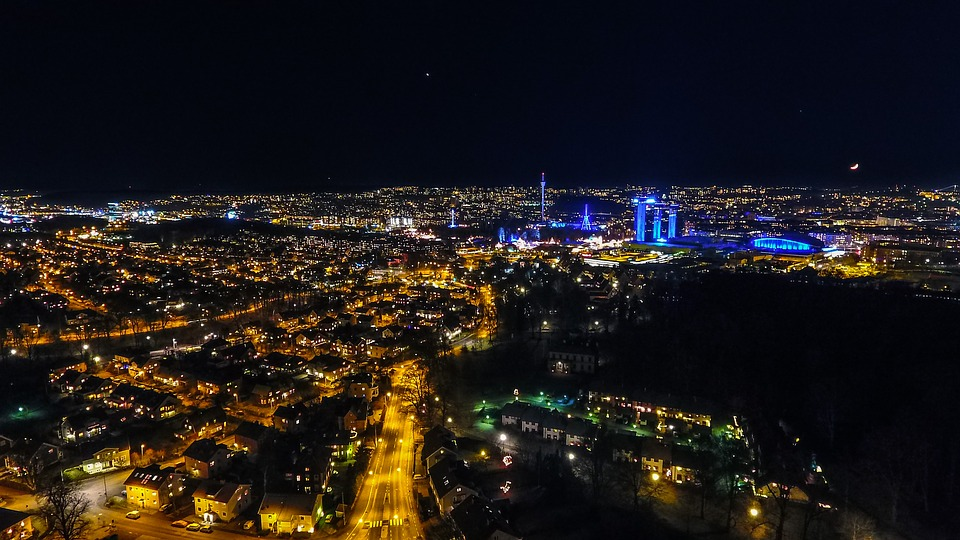
\includegraphics[height=7cm]{irodalom_res/night_life.jpg}
        \caption{Éjszakai város látképe} %cite{}
    \end{figure}
    
    Az általam készített termékkel főként háztartásokban lévő okos világítás megvalósítása a cél, minél energia gazdaságosabb módon. Erre a legmegfelelőbb technológia a LED világítás.
    
    \subsection{LED világítás és előnyei} %https://www.energy.gov/energysaver/save-electricity-and-fuel/lighting-choices-save-you-money/led-lighting
    
    A fényt kibocsájtó diódák (angolul: light-emitting diode - LED) a mai legenergiatakarékosabb és leggyorsabban fejlődő világítástechnológiák közzé tartoznak. Általánosságban igaz az, hogy a LED-es izzók tovább bírják, ellenállóbbak és hasonló vagy még jobb minőségű megvilágítást biztosítanak, mint más fényforrások.
    
    \begin{figure}[h!] %https://en.wikipedia.org/wiki/Light-emitting_diode
        \centering
        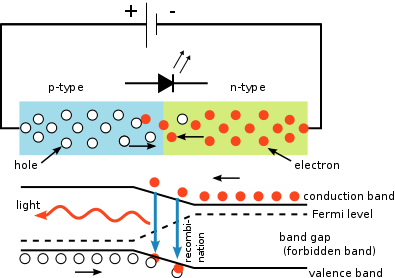
\includegraphics[height=6cm]{irodalom_res/led_working_principle.png}
        \caption{LED működési elve - angolul} %cite{}
    \end{figure}
    Egy pár előnye a LED-es világításoknak:
        \subsubsection{Energiatakarékosság} %https://www.energy.gov/energysaver/save-electricity-and-fuel/lighting-choices-save-you-money/led-lighting
            A LED-es izzók legalább 75\%-al kevesebb energiát használnak és 25x hosszabb ideig bírják, mint a hagyományos izzólámpák. A LED-es izzók elterjedése lenne az egyik legnagyobb hatással az energiatakarékosságra. Az USA-ban például ezzel 2027-ig 348 $TWh$ elektromos munkát (egy éves teljesítménye 44, egyenként 100 Megawattos erőműnek) spórolhatnánk meg, ahhoz képpest ha nem használnánk egyátalán LED-es izzókat, ami több mint 30 milliárd dollár lenne.
            
            A hagyományos izzók teljes teljesítményének 90\%-ából hő termelődik, ami azt jelenti hogy csak 10\%-a fordítódik fénykibocsátásra. A LED-ek esetében alig termelődik hő.
        \subsubsection{Jó színvisszaadás}
            A színvisszaadási index, röviden 'CRI' (Color Rendering Index), a fényforrás azon képességét méri, hogy különféle tárgyakat megvilágítva vele, mennyire képes azok színét visszaadni. %https://hu.wikipedia.org/wiki/Sz%C3%ADnvisszaad%C3%A1s
             \begin{figure}[h!] %https://www.eledlights.com/blog/post/color-temperature-color-rendering-index-what-the-numbers-tell-you/
                \centering
                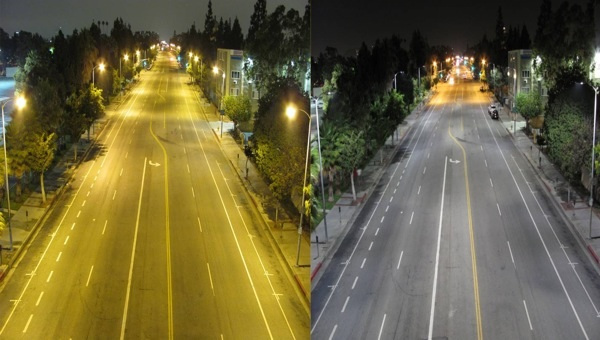
\includegraphics[height=6cm]{irodalom_res/cri_los_angeles.jpg}
                \caption{Utcai megvilágítás kisnyomású nátriumlámpával és LED-del} %cite{}
             \end{figure}
             
        \subsubsection{Környezetbarát}
            A higanylámpával és a fénycsővel ellentétben, a LED-es megoldások nem tartalmaznak higanyt.
        \subsubsection{Széles működési tartomány}
            A LED-k jól hidegben és melegben is egyaránt jól funkcionálnak, működésükhöz esetekben nagyon kis feszültségek is elegendőek, ezáltal alkalmas kültéri megvilágításokra is.
    
    \subsection{Forgalomban lévő eszközök áttekintése //TODO}
        Manapság rengeteg gyártó kínál hasonló okos világítás rendszereket, amelyek közül szeretnék bemutatni egy párat.\\
                            
        miert is jok ezek? \\
        %https://www.cnet.com/how-to/why-your-next-light-bulb-should-be-a-smart-bulb/
        %https://www.pcmag.com/article2/0,2817,2483488,00.asp
        %pro con
        %https://www.the-ambient.com/reviews/the-best-smart-lights-bulbs-platforms-209
            állítható fényerősség\\
            bárhonnan vezérelehők\\
            színtváltók\\
            akár zenét is lejátszanak\\
            
        
        \subsubsection{Phillips HUE} %https://www2.meethue.com/en-us
            központ kell hozzá\\
            
            általános foglalatba csavarható izzók + mások\\
            kinti benti világítás\\
            zenére világítás\\
            hanggal vezérelhetőség\\
            
            
        \subsubsection{LIFX} 
            általános foglalatba becsavarható\\
            ledszalag\\
            csempés\\
        
        \subsubsection{tplink korte}%https://www.amazon.de/TP-Link-Gl%C3%BChbirne-funktioniert-warmwei%C3%9F-erforderlich/dp/B01N3634DR/ref=sr_1_9?ie=UTF8&qid=1542973740&sr=8-9&keywords=SMART%2BLIGHT&th=1
            
        
        \subsubsection{Általásnos vezérelhető LED szalag}%https://www.amazon.de/dp/B0799FFFY7/ref=sspa_dk_detail_4?psc=1&pd_rd_i=B0799FFFY7&pf_rd_m=A3JWKAKR8XB7XF&pf_rd_p=00903874-3af0-47e0-8622-ee58087f71cf&pd_rd_wg=ikWca&pf_rd_r=E2ANMKZA4S6GBYDQ5CGH&pf_rd_s=desktop-dp-sims&pf_rd_t=40701&pd_rd_w=s42m4&pf_rd_i=desktop-dp-sims&pd_rd_r=408ef61c-ef16-11e8-8bb0-a509d9a0f381
        

\end{document}

